\chapter{Geometric Transformations}
\label{ch:lesson08}

This chapter covers how to move, resize, and reshape images: flipping, cropping, rotating, and scaling, and then the more general hierarchy of 2D transformations --- \textbf{Euclidean}, \textbf{similarity}, and \textbf{affine} --- that those operations are all special cases of.

\section{A test image with no symmetry}

A letter ``F'' (Figure~\ref{fig:l08-1}) has no rotational or mirror symmetry --- every flip and rotation produces a visibly different result, which makes it easy to tell the transformations apart.

\begin{figure}[h]
\centering
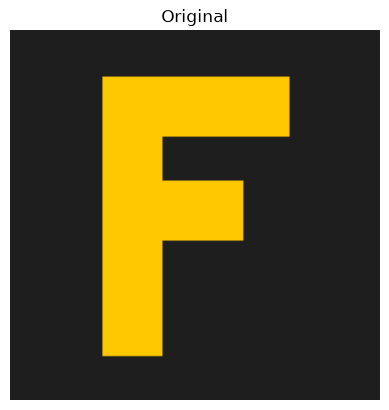
\includegraphics[width=0.3\textwidth]{figures/lesson08_fig01.png}
\caption{The test image: an asymmetric letter F.}
\label{fig:l08-1}
\end{figure}

\section{Basic operations}

Some basic operations:

\textbf{Flipping.} \code{cv2.flip} mirrors an image: code \code{1} flips horizontally, \code{0} flips vertically, \code{-1} flips both (Figure~\ref{fig:l08-2}).

\begin{figure}[h]
\centering
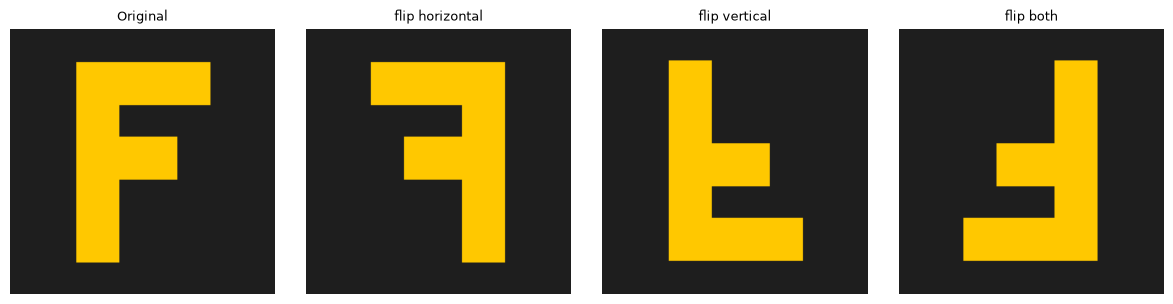
\includegraphics[width=0.9\textwidth]{figures/lesson08_fig02.png}
\caption{Horizontal, vertical, and both-axis flips.}
\label{fig:l08-2}
\end{figure}

\textbf{Cropping} is just array slicing --- no OpenCV function needed: \code{image[y0:y1, x0:x1]} keeps rows \code{y0..y1} and columns \code{x0..x1} (Figure~\ref{fig:l08-3}).

\begin{figure}[h]
\centering
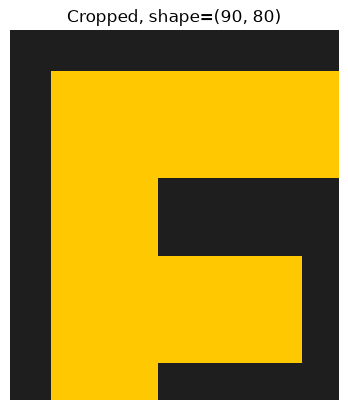
\includegraphics[width=0.3\textwidth]{figures/lesson08_fig03.png}
\caption{A crop, obtained by plain NumPy slicing.}
\label{fig:l08-3}
\end{figure}

\textbf{Scaling (resizing).} \code{cv2.resize} changes an image's dimensions, optionally with different factors for width and height. The ratio of width to height is the \textbf{aspect ratio}. Uniform scaling preserves shape; non-uniform scaling stretches or squashes it.

\begin{lstlisting}
uniform    = cv2.resize(img, None, fx=0.5, fy=0.5)
stretched  = cv2.resize(img, None, fx=1.5, fy=0.6)
\end{lstlisting}

Figure~\ref{fig:l08-4} shows both.

\begin{figure}[h]
\centering
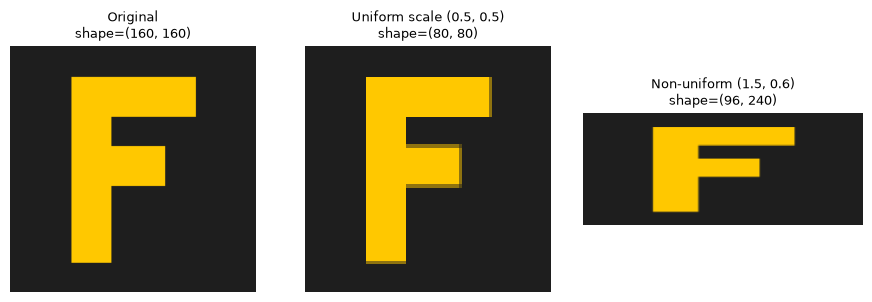
\includegraphics[width=0.85\textwidth]{figures/lesson08_fig04.png}
\caption{Uniform scaling preserves aspect ratio; non-uniform scaling does not.}
\label{fig:l08-4}
\end{figure}

\textbf{Rotating.} \code{cv2.getRotationMatrix2D} builds a $2\times3$ matrix for rotating by an arbitrary angle around a chosen center, which \code{cv2.warpAffine} then applies to the image.

\begin{lstlisting}
M = cv2.getRotationMatrix2D(center, angle=25, scale=1.0)
rotated = cv2.warpAffine(img, M, (w, h))
\end{lstlisting}

Figure~\ref{fig:l08-5} shows the result.

\begin{figure}[h]
\centering
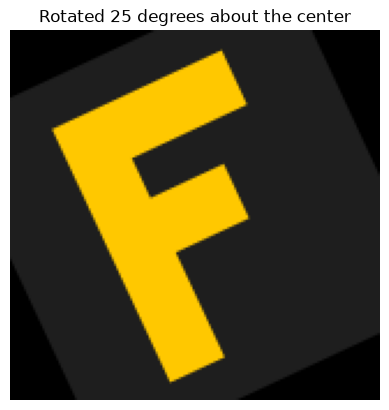
\includegraphics[width=0.3\textwidth]{figures/lesson08_fig05.png}
\caption{Rotation about the image center.}
\label{fig:l08-5}
\end{figure}

\section{The transformation hierarchy}

Flipping, rotating, scaling, and translating are all instances of a general $2\times3$ matrix transform
\begin{equation}
\begin{bmatrix}x'\\y'\end{bmatrix} = \begin{bmatrix}a & b\\c & d\end{bmatrix}\begin{bmatrix}x\\y\end{bmatrix} + \begin{bmatrix}t_x\\t_y\end{bmatrix}
\end{equation}
applied with \code{cv2.warpAffine}. Restricting the $2\times2$ part in different ways gives a nested family of transformations, from most to least restrictive:

\begin{center}
\begin{tabular}{lll}
\hline
\textbf{Transform} & \textbf{Free parameters} & \textbf{Preserves} \\
\hline
Euclidean (rigid) & rotation $\theta$, translation & lengths, angles \\
Similarity & \quad + uniform scale $s$ & angles, ratios of lengths \\
Affine & any invertible $2{\times}2$ matrix & parallelism, ratios along a line \\
\hline
\end{tabular}
\end{center}

Two things change going down the table, in opposite directions. The \emph{set of allowed transforms} grows: every Euclidean transform is a special case of a similarity transform (just $s=1$), and every similarity transform is a special case of an affine transform (just a rotation-and-scale matrix instead of an arbitrary one). In exchange for that extra flexibility, the \emph{properties guaranteed to survive} shrink: Euclidean preserves both lengths and angles; similarity gives up preserving lengths themselves (only their ratios survive); affine gives up angles too. Affine transforms are the most general of the three: they can shear a square into a parallelogram, something neither Euclidean nor similarity transforms can do, as Figure~\ref{fig:l08-6} shows.

\begin{figure}[h]
\centering
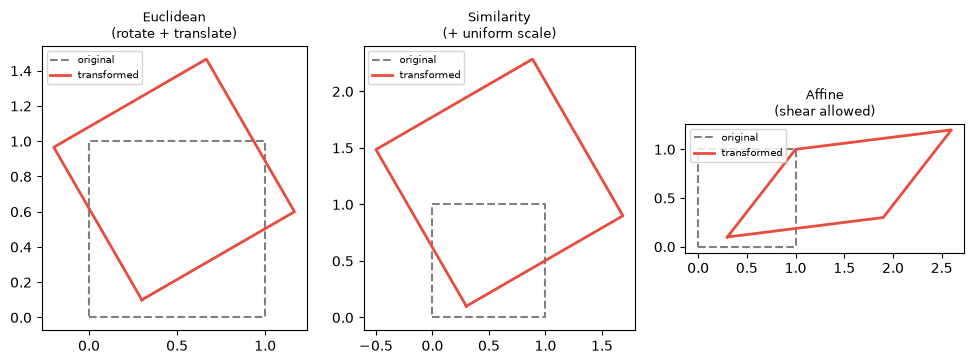
\includegraphics[width=0.85\textwidth]{figures/lesson08_fig06.png}
\caption{A unit square under each transform. Only the affine square stops looking like a (possibly resized) square --- its corners are no longer $90^\circ$, because affine transforms allow shear. All three keep opposite sides parallel. (The more general projective transforms, e.g.\ camera perspective, are covered in a later chapter.)}
\label{fig:l08-6}
\end{figure}

\subsection*{Fitting an affine transform from point correspondences}

In practice we often don't know the transform matrix directly --- e.g., a flat object was photographed \emph{at an angle}, and we want to undo the distortion. This requires identifying a few landmark points in both the crooked photo and where they \emph{should} be in a canonical, front-on view. \code{cv2.getAffineTransform} takes 3 such point correspondences (the minimum needed to determine all 6 affine parameters) and returns the matrix that maps one set onto the other --- solve for the warped-to-canonical direction, and applying it \emph{rectifies} the photo.

\begin{lstlisting}
M_recovered = cv2.getAffineTransform(warped_pts, canonical_pts)
rectified = cv2.warpAffine(warped, M_recovered, (w, h))
\end{lstlisting}

Figure~\ref{fig:l08-7} shows the original, the simulated photo, and the rectified result.

\begin{figure}[h]
\centering
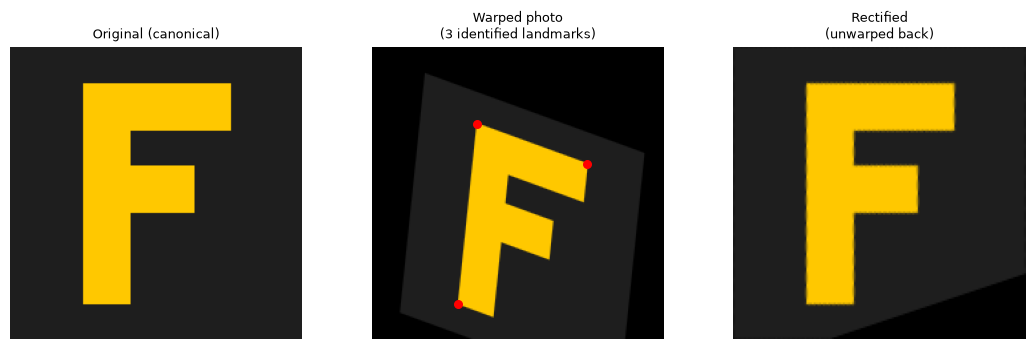
\includegraphics[width=0.95\textwidth]{figures/lesson08_fig07.png}
\caption{Original, a simulated skewed photo with 3 identified landmarks, and the rectified result --- mean absolute pixel error against the true original is just $3.14$ (out of 255).}
\label{fig:l08-7}
\end{figure}

\subsection*{Exercises}
\begin{enumerate}
  \item \code{cv2.flip} is not part of the affine family written in matrix form above (rotation matrices $R$ always have determinant $+1$). What determinant does a flip's $2\times2$ matrix have? Construct the $2\times2$ matrix for \code{flip(1)} and check.
  \item Build a similarity transform matrix with $s=1$ and confirm it matches a pure Euclidean transform --- i.e.\ similarity is a strict generalization of Euclidean, not a different family.
  \item Modify the affine matrix in the unit-square example so that opposite sides are \emph{not} parallel. What has to break for that to happen? (Hint: this is exactly the boundary that separates affine from projective transforms.)
\end{enumerate}

\vfill
\fullcode{lesson08}{lesson08_geometric_transformations}
